\documentclass[12pt, a4paper, oneside]{ctexart}
\usepackage{amsmath, amsthm, amssymb, bm, color, graphicx, geometry, mathrsfs,extarrows, braket, booktabs, array, xcolor, fontspec, appendix, float, subfigure, wrapfig, enumitem}
\usepackage[colorlinks,linkcolor=red,anchorcolor=blue,citecolor=blue,urlcolor=blue,menucolor=black]{hyperref}

%%%% 设置中文字体 %%%%
\setCJKmainfont{方正新书宋_GBK.ttf}[ BoldFont = 方正小标宋_GBK, ItalicFont = 方正楷体_GBK]
%%%% 设置英文字体 %%%%
\setmainfont{Times New Roman}
\setsansfont{Calibri}
\setmonofont{Consolas}

%%%% 设置代码块 %%%%
% 在vscode中使用minted需要先配置python解释器, Ctrl+Shift+P, 输入Python: Select Interpreter选择安装了Pygments的Python版本. 再在setting.json中xelatex和pdflatex的参数中加入 "--shell-escape", 即可
% TeXworks中配置方法参考: https://blog.csdn.net/RobertChenGuangzhi/article/details/108140093
\usepackage{minted}
\renewcommand{\theFancyVerbLine}{
    \sffamily\textcolor[rgb]{0.5,0.5,0.5}{\scriptsize\arabic{FancyVerbLine}}} % 修改代码前序号大小
% 加入不同语言的代码块
\newmintinline{cpp}{fontsize=\small, linenos, breaklines, frame=lines}
\newminted{cpp}{fontsize=\small, linenos, breaklines, frame=lines}
\newmintedfile{cpp}{fontsize=\small, linenos, breaklines, frame=lines}
\newmintinline{matlab}{fontsize=\small, linenos, breaklines, frame=lines}
\newminted{matlab}{fontsize=\small, mathescape, linenos, breaklines, frame=lines}
\newmintedfile{matlab}{fontsize=\small, linenos, breaklines, frame=lines}
\newmintinline{python}{fontsize=\small, linenos, breaklines, frame=lines, python3}  % 使用\pythoninline{代码}
\newminted{python}{fontsize=\small, linenos, breaklines, frame=lines, python3}  % 使用\begin{pythoncode}代码\end{pythoncode}
\newmintedfile{python}{fontsize=\small, linenos, breaklines, frame=lines, python3}  % 使用\pythonfile{代码地址}

%%%% 设置行间距与页边距 %%%%
\linespread{1.2}
\geometry{left=2.5cm, right=2.5cm, top=2.5cm, bottom=2.5cm}

%%%% 定理类环境的定义 %%%%
\newtheorem{example}{例}            % 整体编号
\newtheorem{theorem}{定理}[section] % 定理按section编号
\newtheorem{definition}{定义}
\newtheorem{axiom}{公理}
\newtheorem{property}{性质}
\newtheorem{proposition}{命题}
\newtheorem{lemma}{引理}
\newtheorem{corollary}{推论}
\newtheorem{remark}{注解}
\newtheorem{condition}{条件}
\newtheorem{conclusion}{结论}
\newtheorem{assumption}{假设}
\numberwithin{equation}{section}  % 公式按section编号 (公式右端的小括号)
\newtheorem{algorithm}{算法}

\newsavebox{\nameinfo}
\newenvironment{myTitle}[1]{
    \begin{center}
    {\zihao{-2}\bf #1\\}
    \zihao{-4}\it
}{\end{center}}  % \begin{myTitle}{标题内容}作者信息\end{myTitle}
\newcounter{problem}  % 问题序号计数器
\newenvironment{problem}[1][]{\stepcounter{problem}\par\noindent\textbf{题目\arabic{problem}. #1}}{\smallskip\par}
\newenvironment{solution}[1][]{\par\noindent\textbf{#1解答. }}{\smallskip\par}  % 可带一个参数表示题号\begin{solution}{题号}
\newenvironment{note}{\par\noindent\textbf{注记. }}{\smallskip\par}

%%%% 图片相对路径 %%%%
\graphicspath{{figure/}} % 当前目录下的figure文件夹, {../figure/}则是父目录的figure文件夹
\setlength{\abovecaptionskip}{-0.2cm}  % 缩紧图片标题与图片之间的距离
\setlength{\belowcaptionskip}{0pt} 

%%%% 缩小item,enumerate,description两行间间距 %%%%
\setenumerate[1]{itemsep=0pt,partopsep=0pt,parsep=\parskip,topsep=5pt}
\setitemize[1]{itemsep=0pt,partopsep=0pt,parsep=\parskip,topsep=5pt}
\setdescription{itemsep=0pt,partopsep=0pt,parsep=\parskip,topsep=5pt}

\everymath{\displaystyle} % 默认全部行间公式, 想要变回行内公式使用\textstyle
\DeclareMathOperator*\uplim{\overline{lim}}     % 定义上极限 \uplim_{}
\DeclareMathOperator*\lowlim{\underline{lim}}   % 定义下极限 \lowlim_{}
\DeclareMathOperator*{\argmax}{arg\,max}  % 定义取最大值的参数 \argmax_{}
\DeclareMathOperator*{\argmin}{arg\,min}  % 定义取最小值的参数 \argmin_{}
\let\leq=\leqslant % 简写小于等于\leq (将全部leq变为leqslant)
\let\geq=\geqslant % 简写大于等于\geq (将全部geq变为geqslant)

%%%% 一些宏定义 %%%%
\def\bd{\boldsymbol}        % 加粗(向量) boldsymbol
\def\disp{\displaystyle}    % 使用行间公式 displaystyle(默认)
\def\tsty{\textstyle}       % 使用行内公式 textstyle
\def\sign{\text{sign}}      % sign function
\def\wtd{\widetilde}        % 宽波浪线 widetilde
\def\R{\mathbb{R}}          % Real number
\def\N{\mathbb{N}}          % Natural number
\def\Z{\mathbb{Z}}          % Integer number
\def\Q{\mathbb{Q}}          % Rational number
\def\C{\mathbb{C}}          % Complex number
\def\K{\mathbb{K}}          % Number Field
\def\P{\mathbb{P}}          % Polynomial
\def\N{\mathbb{N}}          % Natural number
\def\Z{\mathbb{Z}}          % Integer number
\def\E{\mathbb{E}}          % Exception
\def\var{\text{Var}}        % Variance
\def\bias{\text{bias}}      % bias
\def\d{\mathrm{d}}          % differential operator
\def\e{\mathrm{e}}          % Euler's number
\def\i{\mathrm{i}}          % imaginary number
\def\re{\mathrm{Re}}        % Real part
\def\im{\mathrm{Im}}        % Imaginary part
\def\res{\mathrm{Res}}      % Residue
\def\L{\mathcal{L}}         % Loss function
\def\O{\mathcal{O}}         % 时间复杂度
\def\wdh{\widehat}          % 宽帽子 widehat
\def\ol{\overline}          % 上横线 overline
\def\ul{\underline}         % 下横线 underline
\def\add{\vspace{1ex}}      % 增加行间距
\def\del{\vspace{-1.5ex}}   % 减少行间距

%%%% 正文开始 %%%%
\begin{document}
\begin{myTitle}{NLP第二次编程作业}
    强基数学002\\
    吴天阳\quad 2204210460,\ 马煜璇\quad 2204220461
\end{myTitle}
\section{实验目的}

使用文本数据集,网址:\url{http://www.cs.cmu.edu/afs/cs/project/theo-11/www/naive-bayes.html}

该数据集中包含两个文本数据集:

\begin{enumerate}
\item
  总数据集\texttt{20\_newsgroups}:包含20种不同的新闻类别,总计共有19997篇文档,每种类别下应该平均有1000份新闻文档.
\item
  子类文档\texttt{mini\_newsgroups}:由第一个总数据集中每种类别的新闻中随机选择100份,总计2000份文档,用于验证算法的准确度.
\end{enumerate}

我们将使用第一个数据集作为训练集,用第二个数据集作为验证集,用于判断模型的准确率. 选取的分类模型包括K近邻和前馈神经网络.
\section{实验原理}
\subsection{K近邻}
首先构建词向量空间$X$,将训练集文本均转化为词向量后得到词向量空间中的子集$G$,对于验证集中的每一个文本也转化为词向量$\bd{x}$,通过选取$X$中距离$\bd{x}$前$K$个距离最小的元素,选取这$K$个中出现次数最高的种类作为预测结果.

由于$K$近邻算法需要选择较好的$K$值,若$K$大小过小,可能发生过拟合现象,$K$大小过大,可能预测效果不好. 所以我们通过多次计算不同的$K$值,选取结果中平均预测率最高$K$值.
\subsection{前馈神经网络}
先将测试集和验证集的文本全部转化为词向量,注意由于验证集是测试集的子集,需要在测试集中将验证集相同的数据删去.

假设词向量维数为$N$,则前馈神经网络的输入层有$N$个神经元,隐藏层设定为1层,神经元个数设置为$32$,由于一共有$20$中类别,所以将输出层神经元个数设置为$20$.\add

隐藏层的激活函数设置为$sigmoid(x) = \frac{1}{1+\e^{-x}}$,输出层使用$softmax$函数将输出转化为概率$softmax(z_i) = \frac{\e^{z_i}}{\sum_{j=1}^{20}z_j}$,最后损失函数选择交叉熵损失函数
\begin{equation*}
    L(y,\hat{y}) = -\sum_{i=1}^{20}y_i\log\hat{y}_i = -y_c\log \hat{y_c}
\end{equation*}
如果当前类别属于第$c$类,则标签对应one-hot向量为$y_i = (\underbrace{0,\cdots, 0, 1}_{c\text{个}},0,\cdots, 0)$,所以才能将损失函数写为后者的形式.
\subsection{实验环境}

\begin{pythoncode}
Python      '3.9.12'
numpy       '1.20.0'
matplotlib  '3.5.1'
nltk        '3.7'
tensorflow  '2.6.0'
\end{pythoncode}

编辑器使用的是Jupyter notebook.
全部代码已上传至\href{https://github.com/wty-yy/LaTex-Projects/blob/main/NLP/hw2/code/main.ipynb}{GitHub}.
\section{实验步骤与结果分析}
\subsection{数据预处理}
\subsubsection{文件读入处理}
将20种文件类型进行编号,并查看内部的文档数目,使用Python3.6以上的路径处理包
\texttt{pathlib} 中 \texttt{Path} 类,对文件路径进行处理:
\begin{pythoncode}
def initDataset(fname, showInfo=True):
    path = Path(fname)  # 将路径转化为Path类
    folds = [f.name for f in path.iterdir() if f.is_dir()]  # 获取文件夹名称
    for id, fold in enumerate(folds):  # 一共有20个文件夹,分别对其内部文件进行处理
        print(f'处理第{id+1}/{len(folds)}个文件夹{fold}中...')
        now = path.joinpath(fold)
        files = [f.name for f in now.iterdir() if f.is_file()]  # 获取当前文件夹内的文件名
        for file in tqdm(files):  # 获取文件文件名
            pathFile = now.joinpath(file)
            with open(pathFile, errors='replace') as f:  # 打开文件进行处理
            #... 文档处理
\end{pythoncode}

通过观察文档内容,可以发现,文档主要是由两部分构成,第一部分为文档的相关信息,而正文与相关信息之间由一个换行符分开,所以我们通过判断第一个换行符,来提取正文部分.

文本格式如下:
\begin{pythoncode}
Xref: ...
Newsgroups: ...
Path: ...
From: ...
Subject: ...
Message-ID: ...
Organization: ...
References: ...
Lines: ...

In article <C51C4r.BtG@csc.ti.com> rowlands@hc.ti.com (Jon Rowlands) writes:
... 以下都是正文
\end{pythoncode}

文本文件预处理代码:
\begin{pythoncode}
with open(pathFile, errors='replace') as f:  # 打开文件进行处理
    s = f.readline()
    while s != "\n":  # 先找到第一个换行符,下面则是正文
        s = f.readline()
        text = f.read()    
\end{pythoncode}

\subsubsection{分词操作}

首先将20类的文档全部读入,将数据的主要成分提取出来,然后利用NLTK库的分词功能

\begin{enumerate}
\item
  将文章转化为小写 \texttt{words.lower()}
\item
  划分 \texttt{nltk.word\_tokenize(words)}
\item
  标点符号去除,用正则表达式判断单词中是否包含英文,若不包含则删去
\item
  去除停用词,利用
  \texttt{nltk.corpus.stopwords(\textquotesingle{}english\textquotesingle{})}
  获得停用词词库
\item
  词干提取,使用 \texttt{nltk.stem.porter.PorterStemmer(word)}
  词干提取方法
\item
  词性还原,使用 \texttt{nltk.stem.WordNetLemmatizer(word)} 还原词性
\end{enumerate}
\begin{pythoncode}
def extractWords(words):  # 提取分词
    words = words.lower()
    words = word_tokenize(words)  # 分词
    dropWords = ["n't"]  # 这个是计算结果中出现次数第一的,但明显不重要
    words = [word for word in words if re.match(r'[A-Za-z]', word) and word not in dropWords]  # 保证单词中必须包含字母
    stops = set(stopwords.words('english'))
    words = [word for word in words if word not in stops]
    tmp = []  # 词干提取+还原词性
    for word in words:
        stem = PorterStemmer().stem(word)  # 词干提取
        pos = ['n', 'v', 'a', 'r', 's']  # 名词,动词,形容词,副词,附属形容词
        for p in pos:
            stem = WordNetLemmatizer().lemmatize(stem, pos=p)
        tmp.append(stem)  # 还原词性,附属形容词
    words = tmp
    return words
\end{pythoncode}
数据集 \texttt{20\_newsgroups}
提取出的全部数据的相关信息,分别为:类别,编号,文件数,分词数目,词频出现次数最高的前5个词.
\begin{figure}[htbp]
    \hspace*{-1.2cm}
    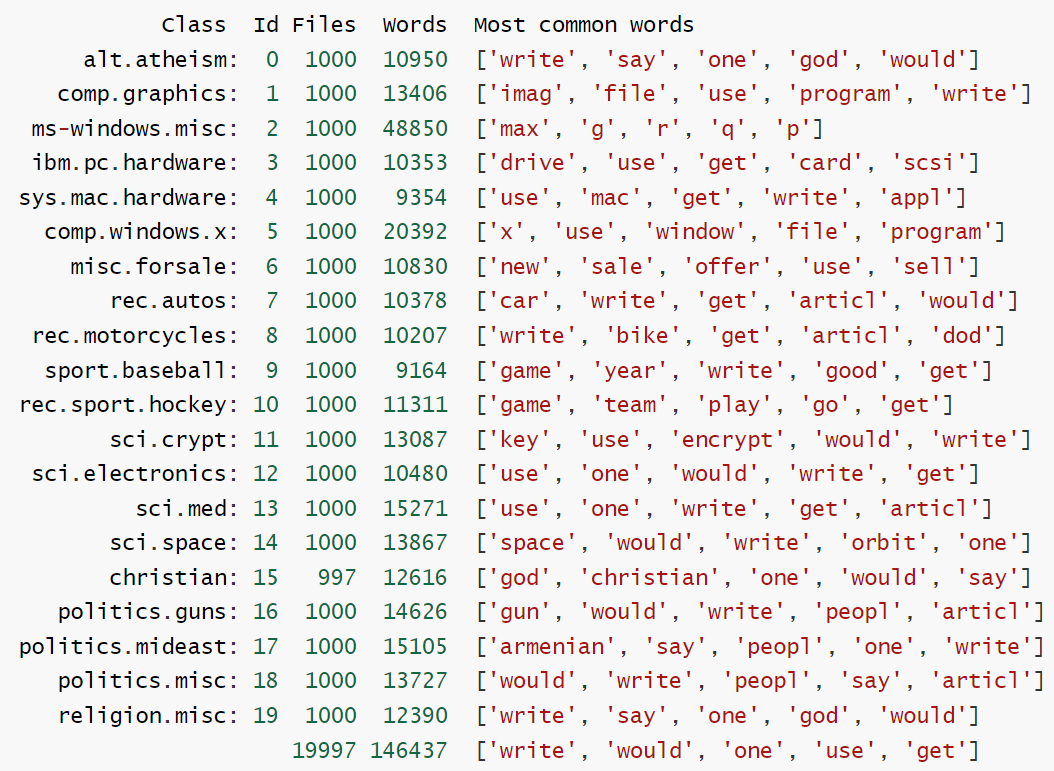
\includegraphics[scale=0.5]{训练集相关信息.png}
\end{figure}

\subsection{分类模型}
\subsubsection{K近邻}
选择前1000个出现频率最高的单词作为词向量的基,这里列出部分词作为基:

\begin{pythoncode}
write, would, one, use, get, articl, say, know, like, think, make, peopl, good, go, time, x, see, also, could, work, u, take, right, new, want, system, even, way, year, thing, come, well, find, may, give, look, need, god, problem, much, mani, tri, first, two, file, mean, max, believ, call, run, question, point, q, anyon, post, seem, program, state, window, tell, differ, r, drive, read, realli, someth, plea, includ, g, sinc, thank...
\end{pythoncode}

将文档转化为词向量,单位化到100,由于总共有1000维,如果单位化为1,每一位大小过小,产生精度问题.

\begin{pythoncode}
def word2vector(word):  # 通过文档生成词向量
    x = np.ones(N)  # 初始化全为1,正则化向量,保证没有0分量
    for t in w:
        if t in word2num:
            x[word2num[t]] += 1
    x /= x.sum() / 100
    return x
\end{pythoncode}
\begin{pythoncode}
# KNN算法
def KNN(word, K=[4]):  # word为原始文档,K可以是一个list,包含多个K值,返回不同K值的预测结果
    now = word2vector(word)  # 获得当前文档的词向量
    dist = []
    for x, y in data:
        dist.append((np.linalg.norm(now - x), y))  # 计算欧氏距离
    dist = sorted(dist, key=(lambda x: x[0]))  # 递增排序
    ret = []
    for k in K:
        tmp = dist[1:k+1]  # 获得前k个,由于原数据集包含当前数据,第0个必然是自身,所以跳过第0个
        classify = [c[1] for c in tmp]
        ret.append(collections.Counter(classify).most_common()[0][0])  # 找到出现次数最多的类别作为预测值
    return np.array(ret)
\end{pythoncode}
计算不同的K值求解正确率,取平均正确率最高的一组,此处设定了几种K的取值:
\begin{pythoncode}
K = [1,2,3,4,5,6,7,8,9,10, 20, 50, 100]
K=1, 正确率: 58.00%
K=2, 正确率: 58.00%
K=3, 正确率: 56.40%
K=4, 正确率: 55.85%
K=5, 正确率: 54.10%
K=6, 正确率: 52.50%
K=7, 正确率: 51.60%
K=8, 正确率: 50.30%
K=9, 正确率: 48.75%
K=10, 正确率: 48.20%
K=20, 正确率: 42.70%
K=50, 正确率: 37.25%
K=100, 正确率: 33.55%
\end{pythoncode}
\begin{figure}[htbp]
    \centering
    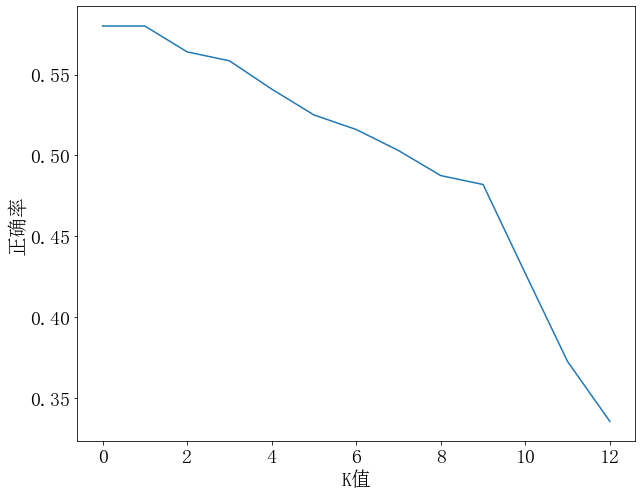
\includegraphics[scale=0.5]{note.figure/不同K值正确率曲线.png}
\end{figure}
我们发现K越小正确率越高,但是K过小可能发生过拟合,所以最后选取了K=4

\begin{pythoncode}
K为4时, 平均正确率较高55.85%
第  1 组类别, 正确率: 0.43
第  2 组类别, 正确率: 0.55
第  3 组类别, 正确率: 0.51
第  4 组类别, 正确率: 0.38
第  5 组类别, 正确率: 0.56
第  6 组类别, 正确率: 0.44
第  7 组类别, 正确率: 0.42
第  8 组类别, 正确率: 0.46
第  9 组类别, 正确率: 0.67
第 10 组类别, 正确率: 0.57
第 11 组类别, 正确率: 0.70
第 12 组类别, 正确率: 0.62
第 13 组类别, 正确率: 0.51
第 14 组类别, 正确率: 0.57
第 15 组类别, 正确率: 0.57
第 16 组类别, 正确率: 0.50
第 17 组类别, 正确率: 0.56
第 18 组类别, 正确率: 0.72
第 19 组类别, 正确率: 0.43
第 20 组类别, 正确率: 0.65
\end{pythoncode}

\subsubsection{前馈型神经网络}
使用TensorFlow神经网络框架
\begin{pythoncode}
import tensorflow as tf
import tensorflow.keras as keras
import tensorflow.keras.layers as layers
\end{pythoncode}

构造训练集,并随机打乱,设置batch大小为16,重复原始数据集5次,得到包含
构造训练集,并随机打乱,设置batch大小为16,重复原始数据集5次,得到包含
\(17835\times 5=89175\)
个元素的数据集,每次对其进行训练(原始数据集太小了,放大了5倍)

\begin{pythoncode}
train_x, train_y = [], []
test_x, test_y = [], []
tmp = [w for words in test_words for w  in words]
for i in range(20):
    for w in test_words[i]:  # 测试集
        x = word2vector(w)
        test_x.append(x)
        test_y.append(i)
    for w in words[i]:  # 训练集
        if w not in tmp:  # 训练集元素不能在测试集中出现
            x = word2vector(w)
            train_x.append(x)
            train_y.append(i)
# 转化为np.ndarray的形式
train_x = np.array(train_x)
train_y = np.array(train_y)
test_x = np.array(test_x)
test_y = np.array(test_y)
# 构建为tf.data.Dataset数据类型
train = tf.data.Dataset.from_tensor_slices((train_x, train_y))
train = train.shuffle(10000).batch(16).repeat(5)  # 对数据集进行预处理
test = tf.data.Dataset.from_tensor_slices((test_x, test_y))
\end{pythoncode}

构建神经网络模型,包含一个含有32个神经元的隐藏层,使用sigmoid作为激活函数,softmax函数作为输出层的激活函数,使用交叉熵损失函数.

\begin{pythoncode}
model = keras.Sequential([
    layers.Dense(32, activation='sigmoid', input_shape=[N,]),  # 隐藏层
    layers.Dense(20, activation='softmax')  # 输出层
])
model.compile(optimizer='adam',  # 优化器
             loss = keras.losses.SparseCategoricalCrossentropy(),  # 损失函数
             metrics=['accuracy'])  # 将准确率作为预测指标
history = model.fit(train, epochs=20, validation_data=(test_x, test_y))
\end{pythoncode}

训练20次,得到的损失和准确率如图下图所示,15次以后,验证集准确率基本稳定在70\%,训练集准确率稳定在80\%左右.
下图准确率最终稳定在 70.9\%

\begin{figure}[htbp]
    \centering
    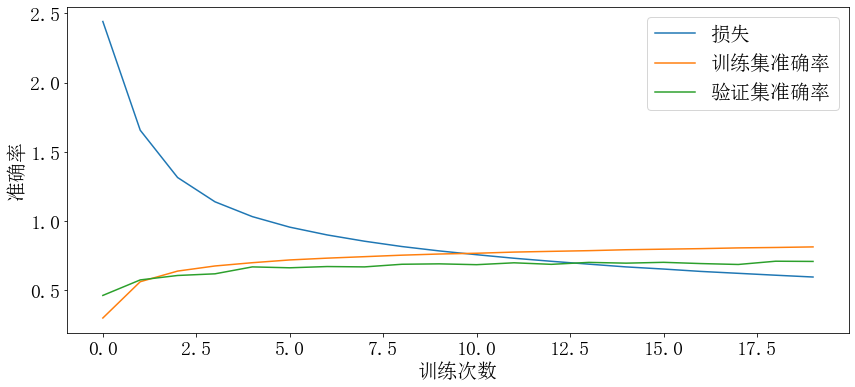
\includegraphics[scale=0.5]{note.figure/神经网络训练过程.png}
\end{figure}

\section{结论与讨论}

通过本次实验,学会了使用 \texttt{nltp}
包对文档进行分词操作,对原式文档进行预处理,使用KNN和前馈神经网络两种不同的模型对文档进行分类预测,正确率分别在55.85\%和70.9\%左右,效果均不是非常好,仍有待改进.

\appendix
\section{附录}
\subsection{神经网络训练日志}
\begin{figure}[htbp]
    \centering
    \hspace*{-2.2cm}
    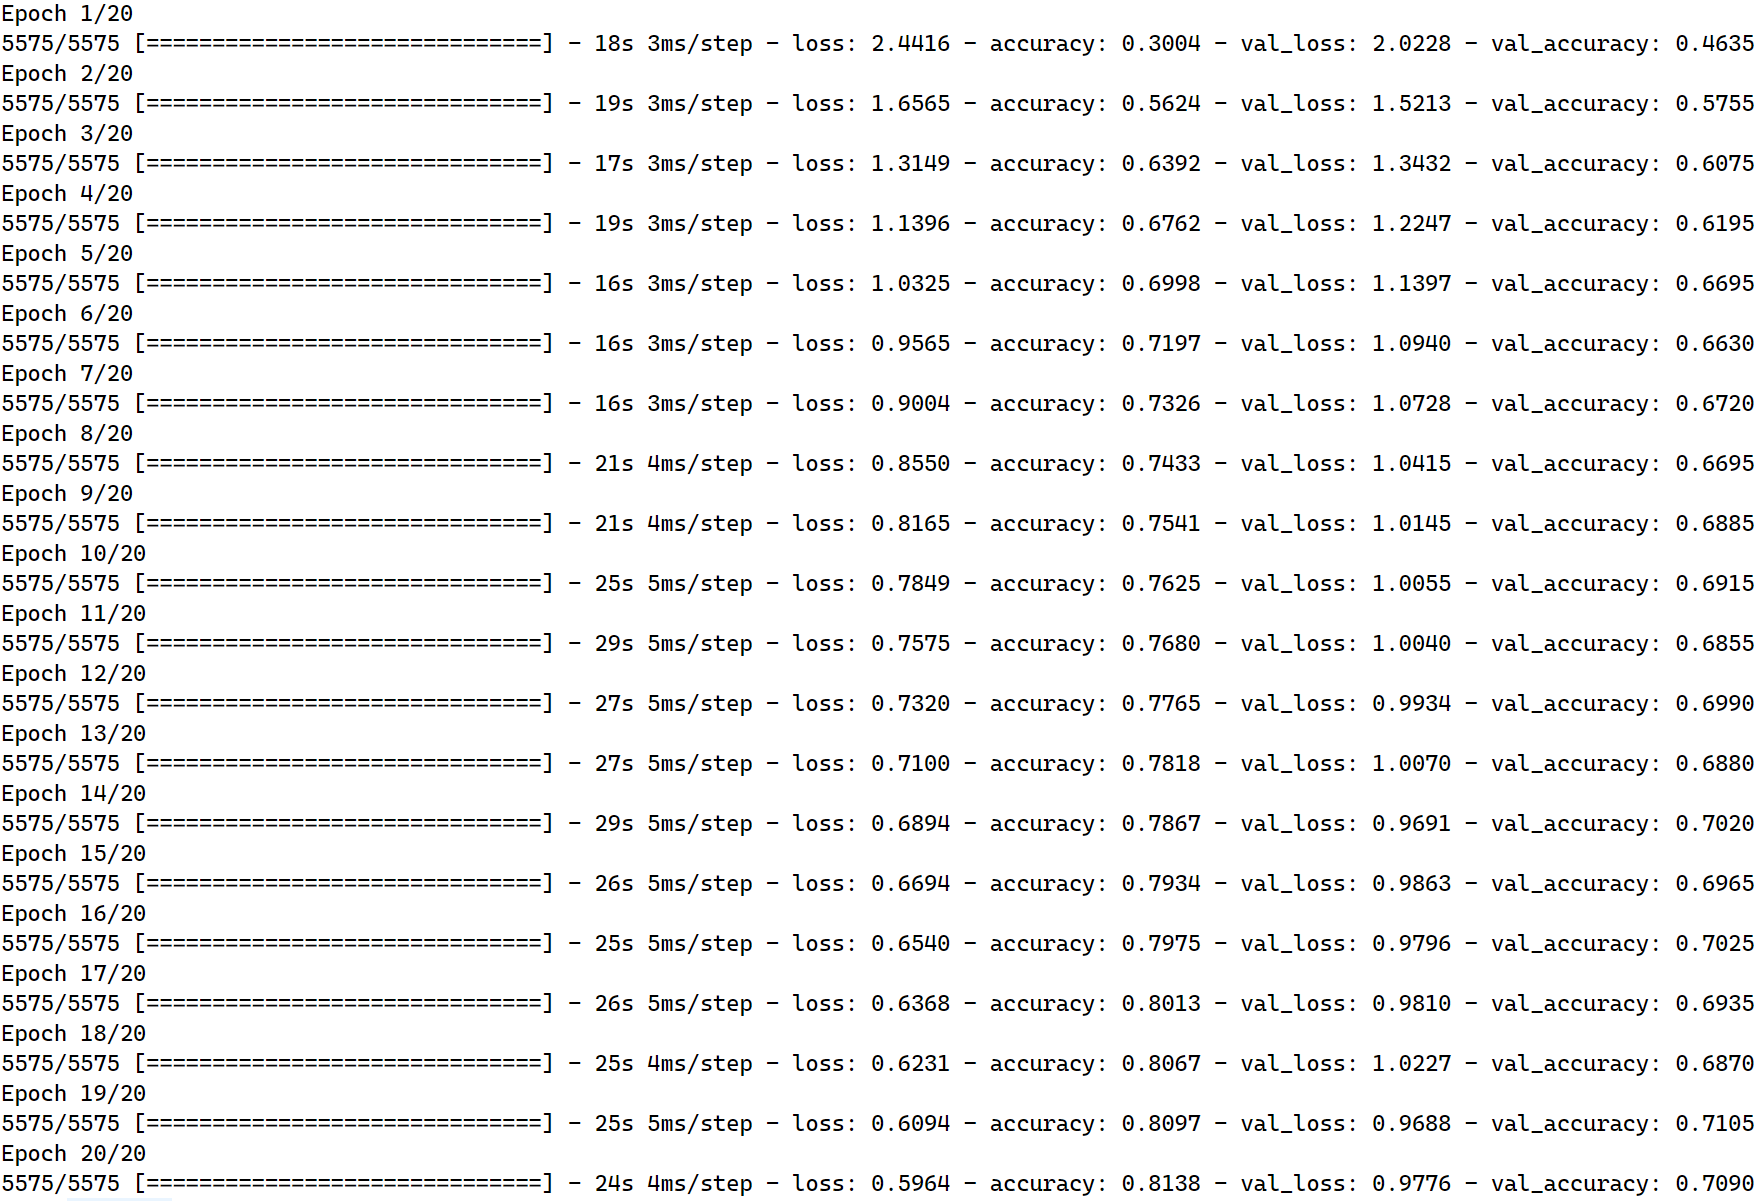
\includegraphics[scale=0.33]{神经网络训练日志.png}
\end{figure}
\end{document}
